
\section{Glioma analysis}

The \sigla{ELMER}{Enhancer Linking by Methylation/Expression Relationship}
tool was used to analyze the molecular differences between the newly
identified G-CIMP-low subtype of glioma that has some regions of the genome with a lower
DNA methylation level and was associated with significantly
worse survival compared to the G-CIMP-high, recently described by Dr. Noushmehr
and his lab \cite{ceccarelli2016molecular}.

For this analysis, TCGA data from the NCI's Genomic Data Commons (GDC) was
downloaded using our R/Bioconductor TCGAbiolinks package described in the previous chapter.
Table \ref{gcimp.samples} summarizes the number of samples in each group that have both \sigla{DNA}{deoxyribonucleic acid}
methylation data for the Illumina HumanMethylation450 platform (HM450) and gene expression data
(RNA-Seq) and Table \ref{gcip.elmer.arg} summarizes the main values for the ELMER arguments.
This analysis was performed with data aligned against the genome of reference hg38 and
using ELMER "supervised" mode, which ensures that in all the steps the
comparisons are made between each group using all their samples.

% Please add the following required packages to your document preamble:
% \usepackage{booktabs}
\begin{table}[h!]
\centering
\caption[G-CIMP analysis: Sample summary]{G-CIMP-high vs G-CIMP-low analysis: number of samples with both DNA methylation (HM450) and gene expression (RNA-seq) data.}
\label{gcimp.samples}
\begin{tabular}{@{}ll@{}}
\toprule
Group       & Number of samples \\ \midrule
G-CIMP-high & 233               \\
G-CIMP-low  & 11
\end{tabular}
\end{table}
% Please add the following required packages to your document preamble:
% \usepackage{booktabs}
\begin{table}[h!]
\centering
\caption[G-CIMP analysis: ELMER arguments values]{G-CIMP-high vs G-CIMP-low analysis: ELMER arguments values.}
\label{gcip.elmer.arg}
\begin{tabular}{@{}lll@{}}
\toprule
Step                        & Argument                           & Value  \\ \midrule
createMAE           & genome &  hg38   \\
Pairs probe-gene correlation/master regulator TF             & Mode &  Supervised   \\
All                         & minSubgroupFrac                    & 100\%  \\
All                         & group1                    & GGimp-high  \\
All                         & group2                    & GGimp-low  \\
All                         & direction                    & hypermethylated probes  \\
DMCs & $\min\Delta\overline{\beta}$                & 0.3    \\
DMCs & p-value adj cut-off                & 0.01   \\
Pair probe-gene correlation           & \# permutations                    & 10000  \\
Pairs  probe-gene correlation           & raw p-value cut-off                & 0.001 \\
Pairs  probe-gene correlation           & empirical p-values cut-off         & 0.001 \\
Motif enrichment            & minimum \# probes  & 10     \\
Motif enrichment            & lower OR                           & 1.1    \\ \bottomrule
\end{tabular}
\end{table}

The DMCs (differently methylated CpGs) analysis, which uses a one-tailed t.test to find
probes with higher mean level in GCIMP-high group compared to the GCIMP-low one.
The result of this analysis is summarized in Figure \ref{fig:gcimpvolcano}.
The volcano plot shows the difference of DNA methylation ($\Delta\overline{\beta}$)
versus significance $-log_{10}(\textrm{FDR corrected P-values})$. Using as defalt cutt-offs
 $\Delta\overline{\beta}\geq0.3$ and $-log_{10}(\textrm{FDR corrected P-values})\leq 0.01$,
$7540$ probes were identified to be differently methylated.

\begin{center}
\begin{figure}[h!]
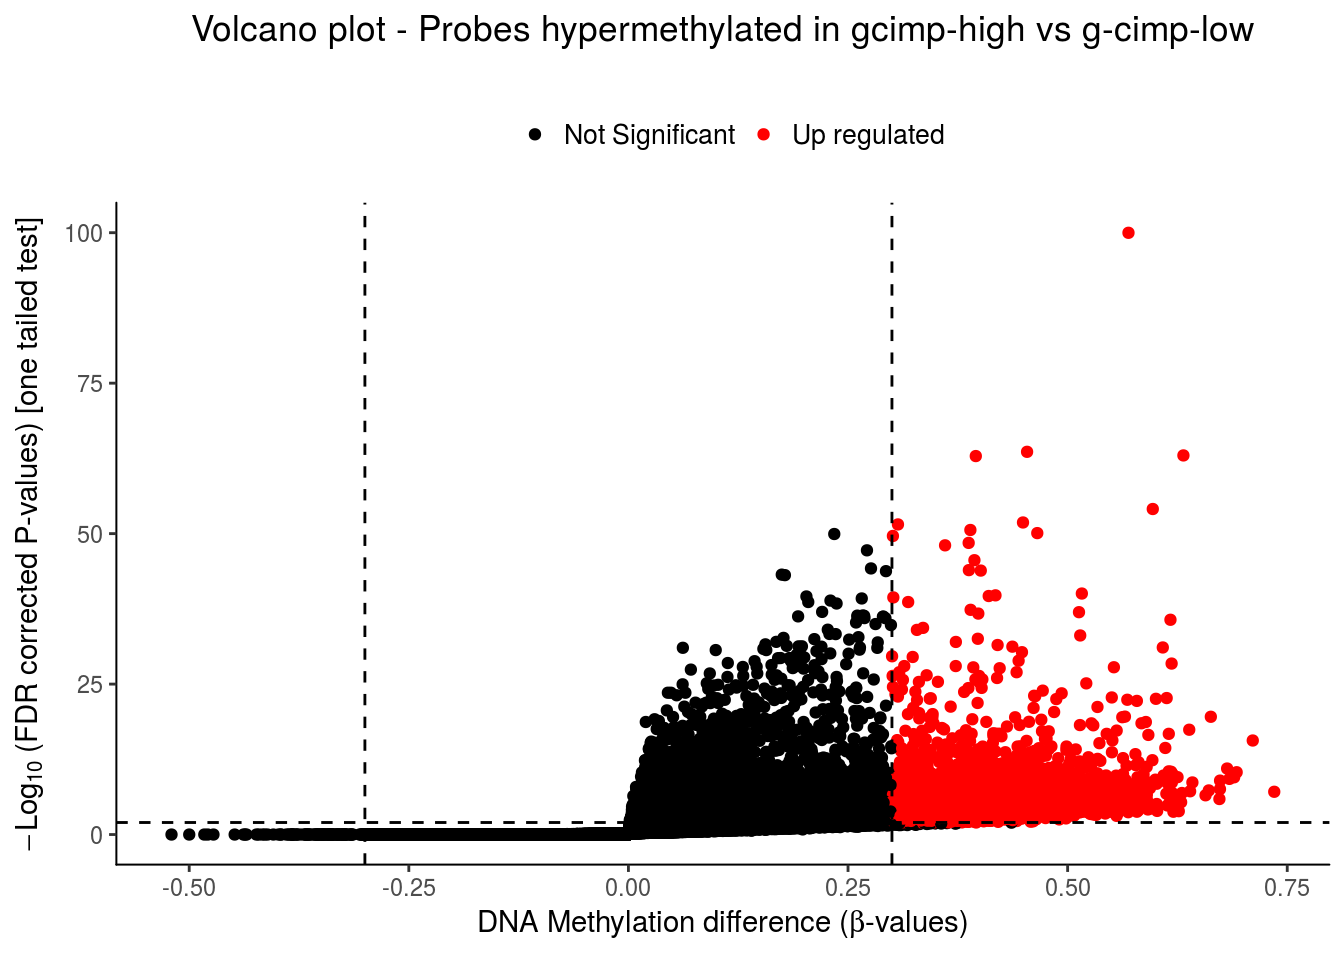
\includegraphics[width=16cm]{images/gcimp_volcano.png}
\caption[G-CIMP analysis: Volcano plot]{\label{fig:gcimpvolcano}G-CIMP analysis: DNA methylation  Volcano plot). Difference of DNA methylation ($\min\Delta\overline{\beta}$) versus significance $-log_{10}(FDR corrected P-values)$.}
\end{figure}

\end{center}

Those differently methylated were then paired with their 10 upstream and 10 downstream genes
and an anti-correlation test which searches for genes highly expressed when the DNA methylation levels
decreases was performed.
Using as cutt-offs
$-log_{10}(\textrm{raw P-values})\leq 0.001$ and $-log_{10}(\textrm{Permutated corrected P-values})\leq 0.001$
for a  $10000$ permutation correction approach,
886 pairs of gene and probes were identified to be anti-correlated.
The result of this analysis is summarized in Figure \ref{fig:gcimpheatmap}.
The heatmap is composed of other three heatmaps, one heatmap for the DNA methylation levels,
one heatmap for the gene expression levels and one with the distance between
the gene and the probe.

\begin{center}
\begin{figure}[h!]

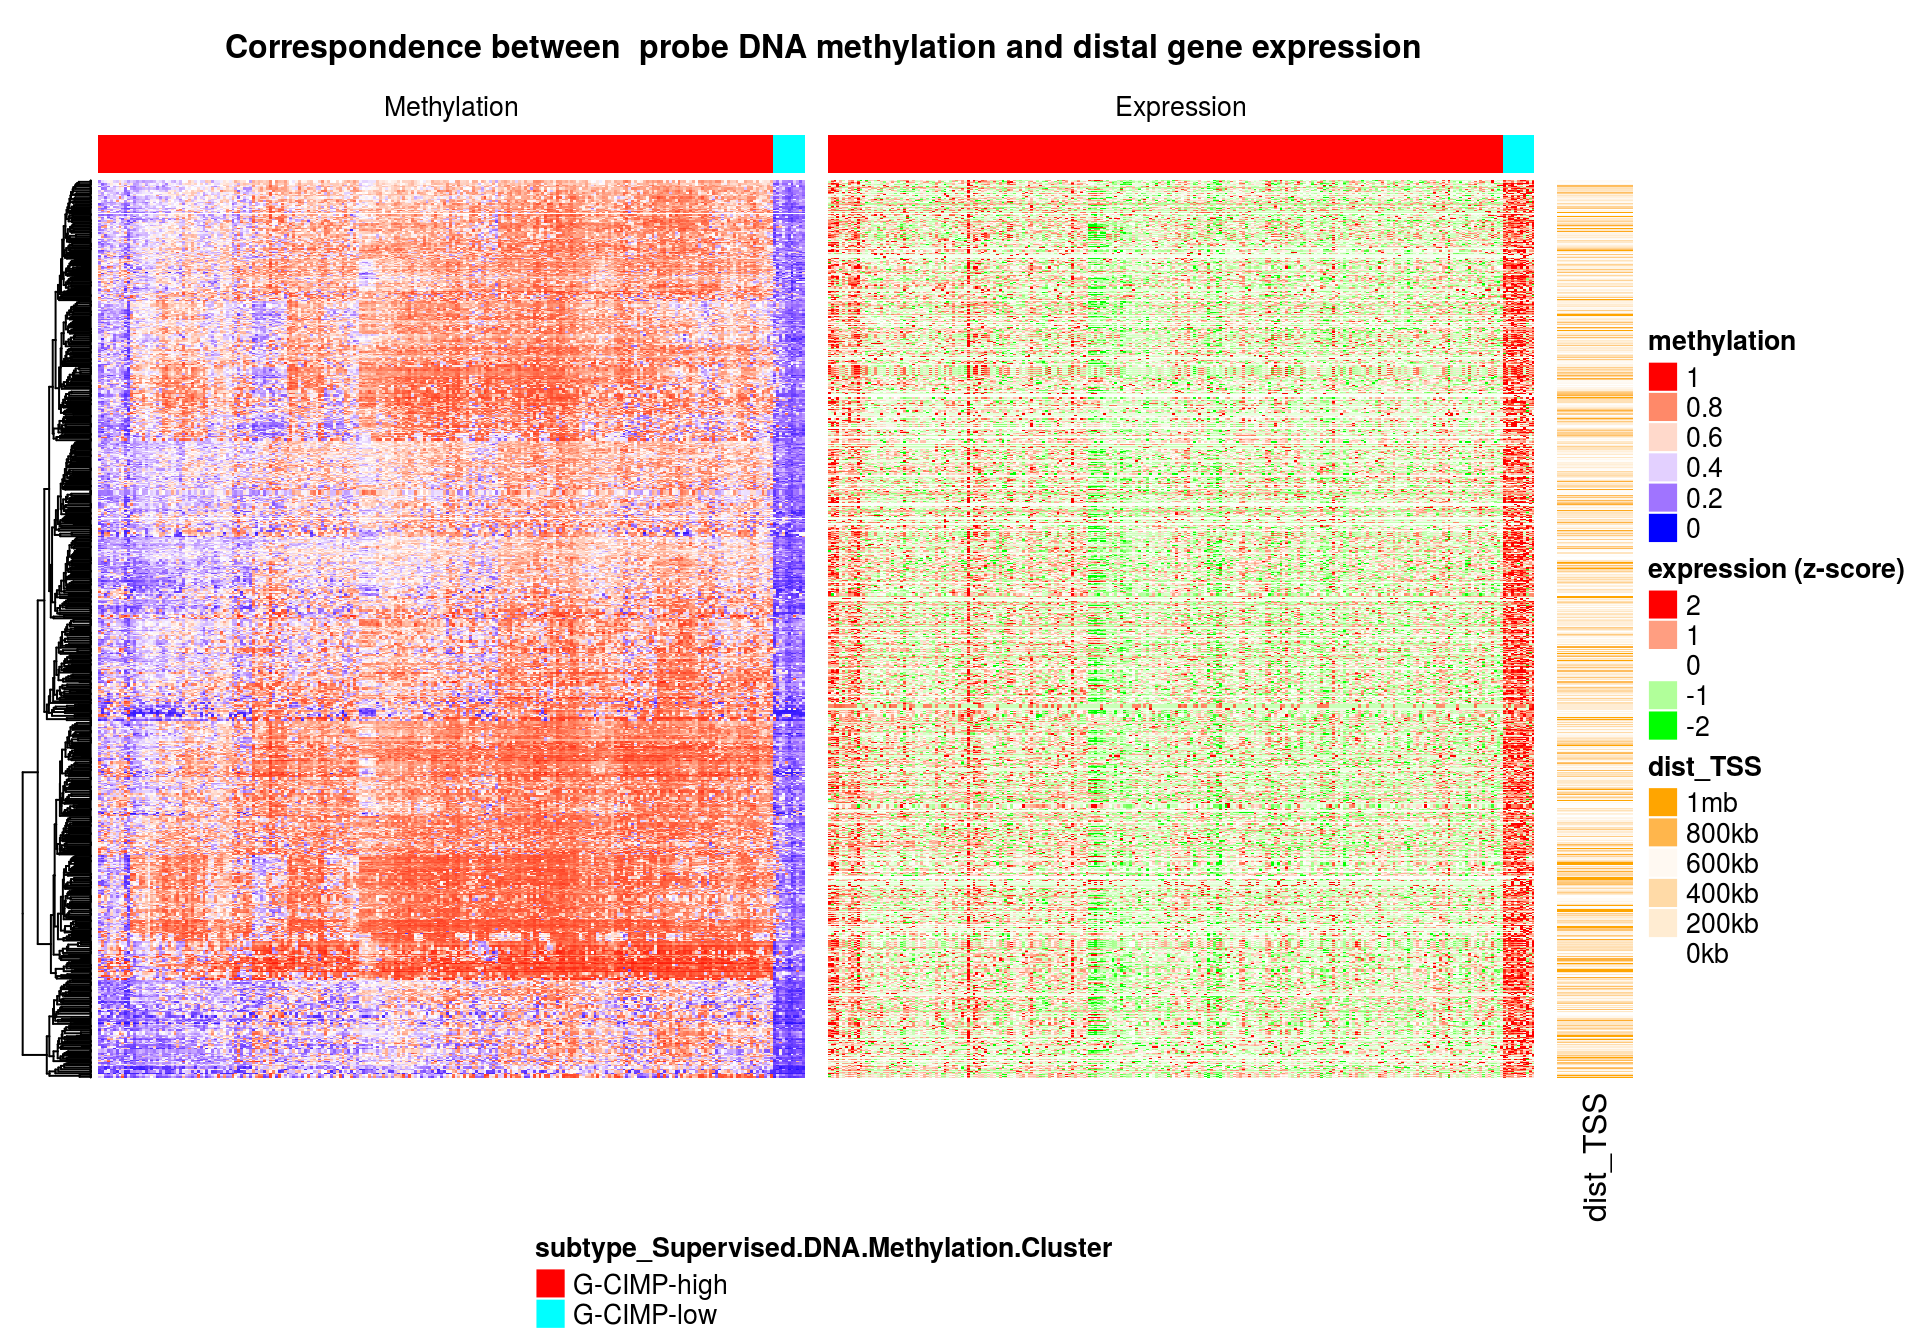
\includegraphics[width=16cm]{images/gcimp_heatmap.png}
\caption[G-CIMP analysis: Heatmap of paired probes and distal genes]{\label{fig:gcimpheatmap}G-CIMP analysis:
Heatmap of paired probes and distal genes. The first heatmap (left one) shows DNA methylation $\beta$ levels ranging from 0 (non-methylated) up to 1 (methylated probes).
The second heatmap (middle one) shows z-scores for gene expression levels (standard deviations from each gene means). The last heatmap (right heatmap) shows the distance between the probe
and gene anti-correlated. The top annotation in the heatmap was retried from \citeonline{cell}}
\end{figure}

\end{center}

\begin{table}[h!]
\centering
\caption[G-CIMP analysis: Summary results]{G-CIMP-high vs G-CIMP-low analysis:
number of distal probes, significant differently methylated probes,
significant anti-correlated paired gene-probes and enriched motifs}
\label{gcimp.summary.results}
\begin{tabular}{@{}ll@{}}
\toprule
Result      & Value \\ \midrule
Distal probes       & 135374 \\
Significant differently methylated probes & 7540               \\
Siginificant anti-correlated paired gene-probes  & 886 \\
Enriched motifs & 84
\end{tabular}
\end{table}

The eriched motifs analysis results are summarized in Figure \ref{tab:or},
which shows the \sigla{OR}{Odds Ratio} (x axis) for the enriched motifs, and in Table  \ref{tab:tf},
which shows the candidate regulatory TFs whose expression anti-correlated
with the DNA methylation level on the probes of each enriched motifs.
 From the most anti-correlated ones, ELMER uses the TFClass
 classification \cite{doi:10.1093/nar/gku1064} to identifies
 which TFs are  known to bind in those motifs.
 This classification has two levels, family and subfamily,
  which groups motifs with a similar signature.
  Depending on the motif, its family classification might have a
  very similar signature, otherwise, the subfamily classification is the most indicated.

\begin{center}
\begin{figure}[h!]
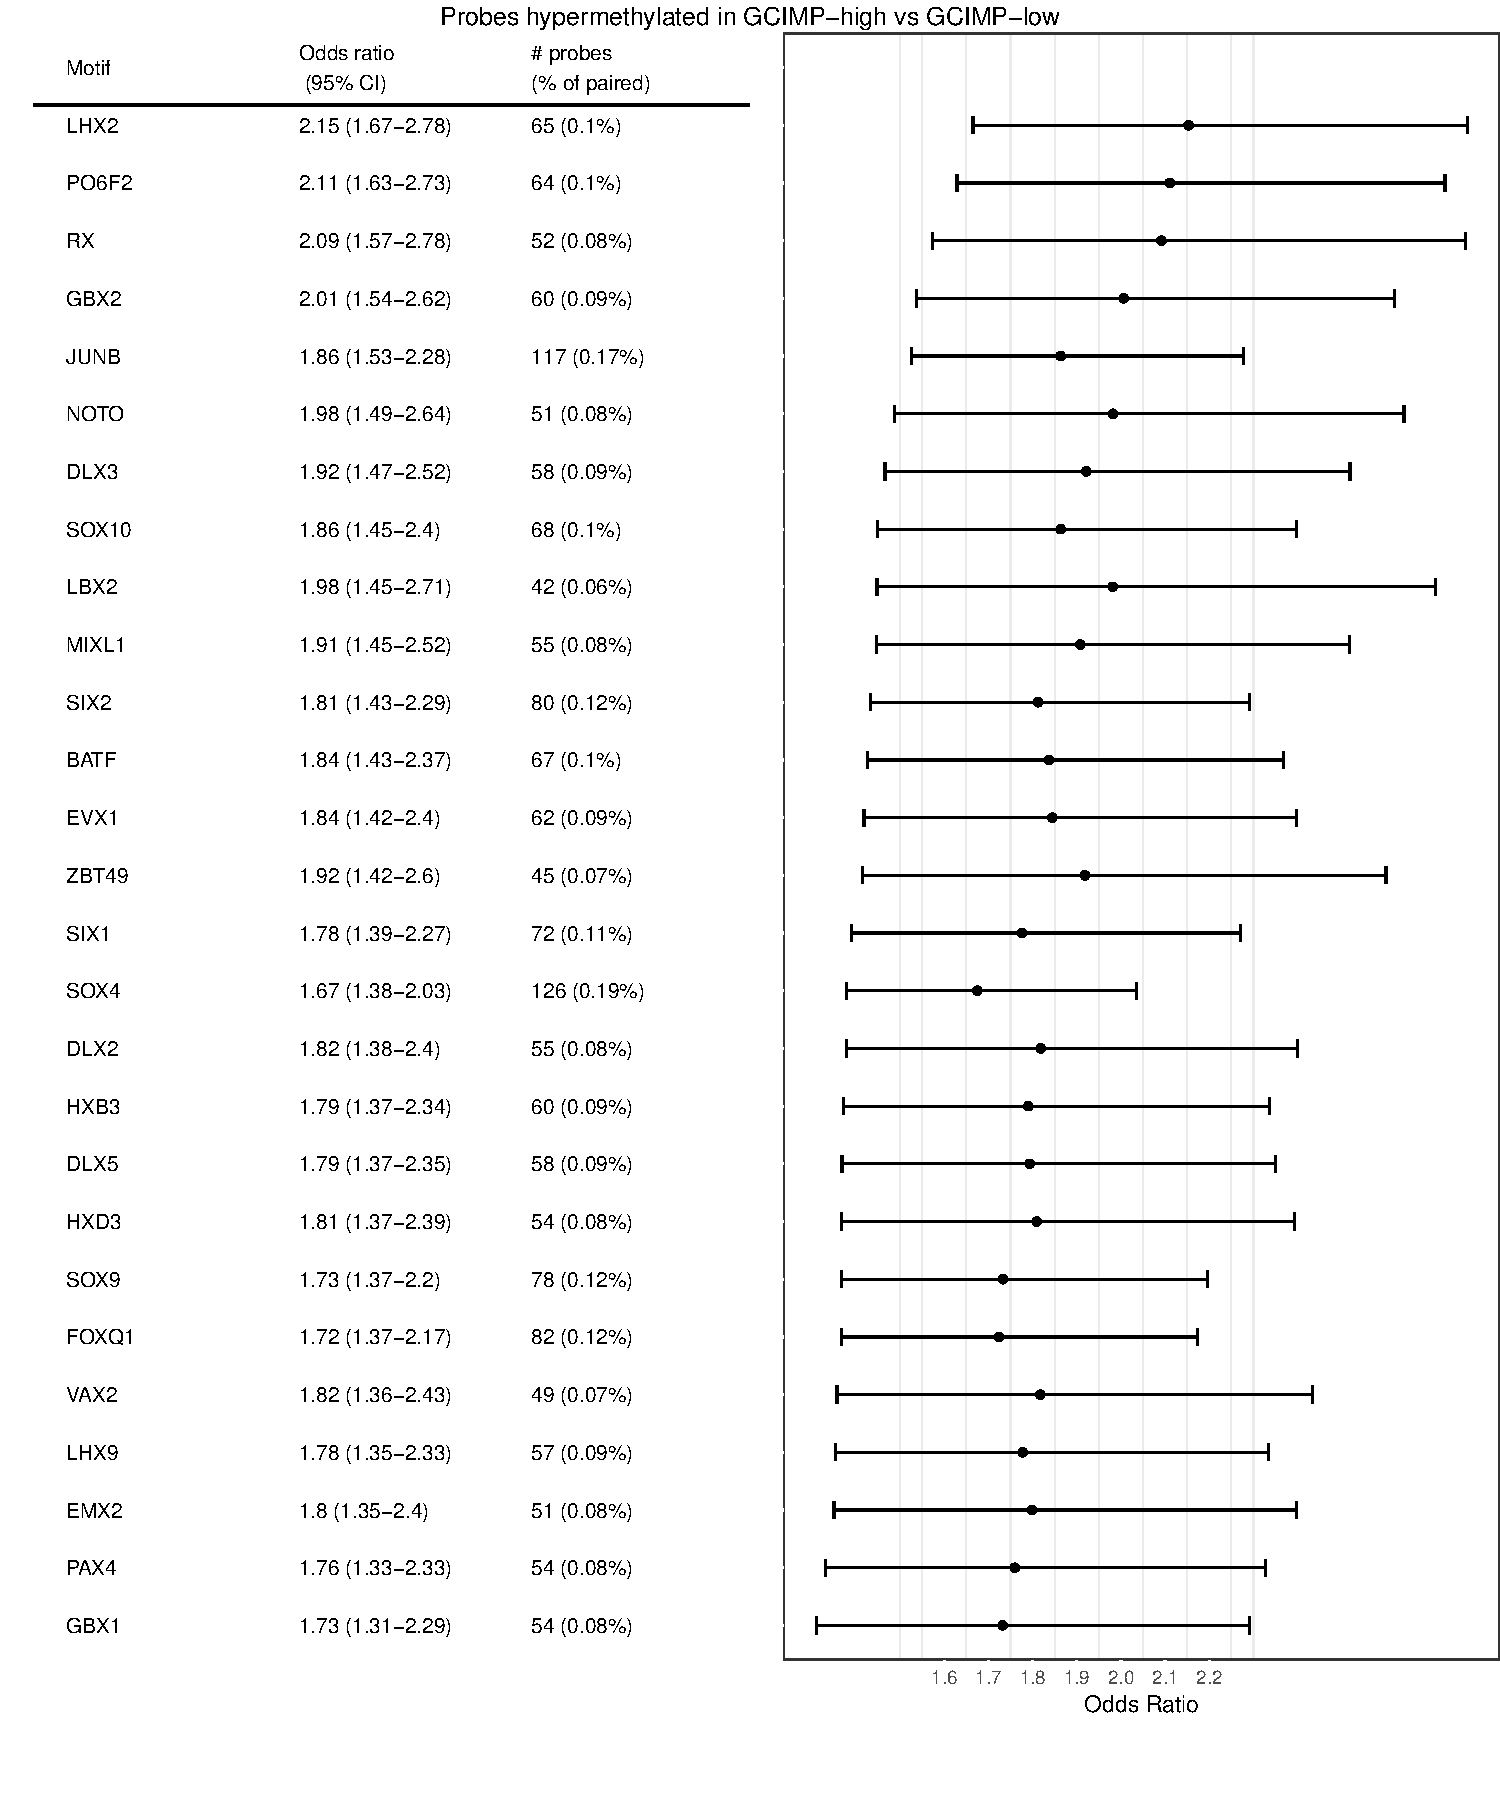
\includegraphics[width=16cm]{images/gcimp_motif_enrichment.pdf}
\caption[G-CIMP analysis: Odds Ratio plot]{\label{tab:or}Motif enrichment analysis: Odds Ratio (x axis) for the selected motifs with lower OR above 1.3. The range shows the 95\% confidence interval for each Odds Ratio.}
\end{figure}

\end{center}


For example, in Table \ref{tab:tf} the motif HXD3 has as potential TF candidate the HOXD13 if we consider the family \sigla{TF}{Transcription Factor} classification and the HOXD3 TF candidate considering the subfamily TF classification. Figure \ref{tab:hocomoco} shows the motif signature for the HOX-related factors family from \sigla{HOCOMOCO}{HOmo sapiens COmprehensive MOdel COllection} database. The transcription factors \sigla{HOXD13}{Homeobox D13} and \sigla{HOXD3}{Homeobox D3} are in the same family (HOX-related factors) but in different subfamilies.



\begin{table}[h!]
\centering
\caption[G-CIMP analysis: TF ranking plot]{TF ranking analysis: statistic For each enriched motif the anti-correlation level of all human TFs expression level with average DNA methylation level at sites with a given motif was access and ranked by the $-log_{10}(P_{value})$, the most relevant one that belongs to the same family as the motif is shown in column \textit{top.potential.TF.family} while the most relevant within the same sub-family classification is shown in column \textit{top.potential.TF.subfamily}}.
\csvautobooktabular[respect underscore]{tables/getTF.hyper.significant.TFs.with.motif.summary.csv}
\label{tab:tf}
\end{table}

\begin{center}
\begin{figure}[h!]
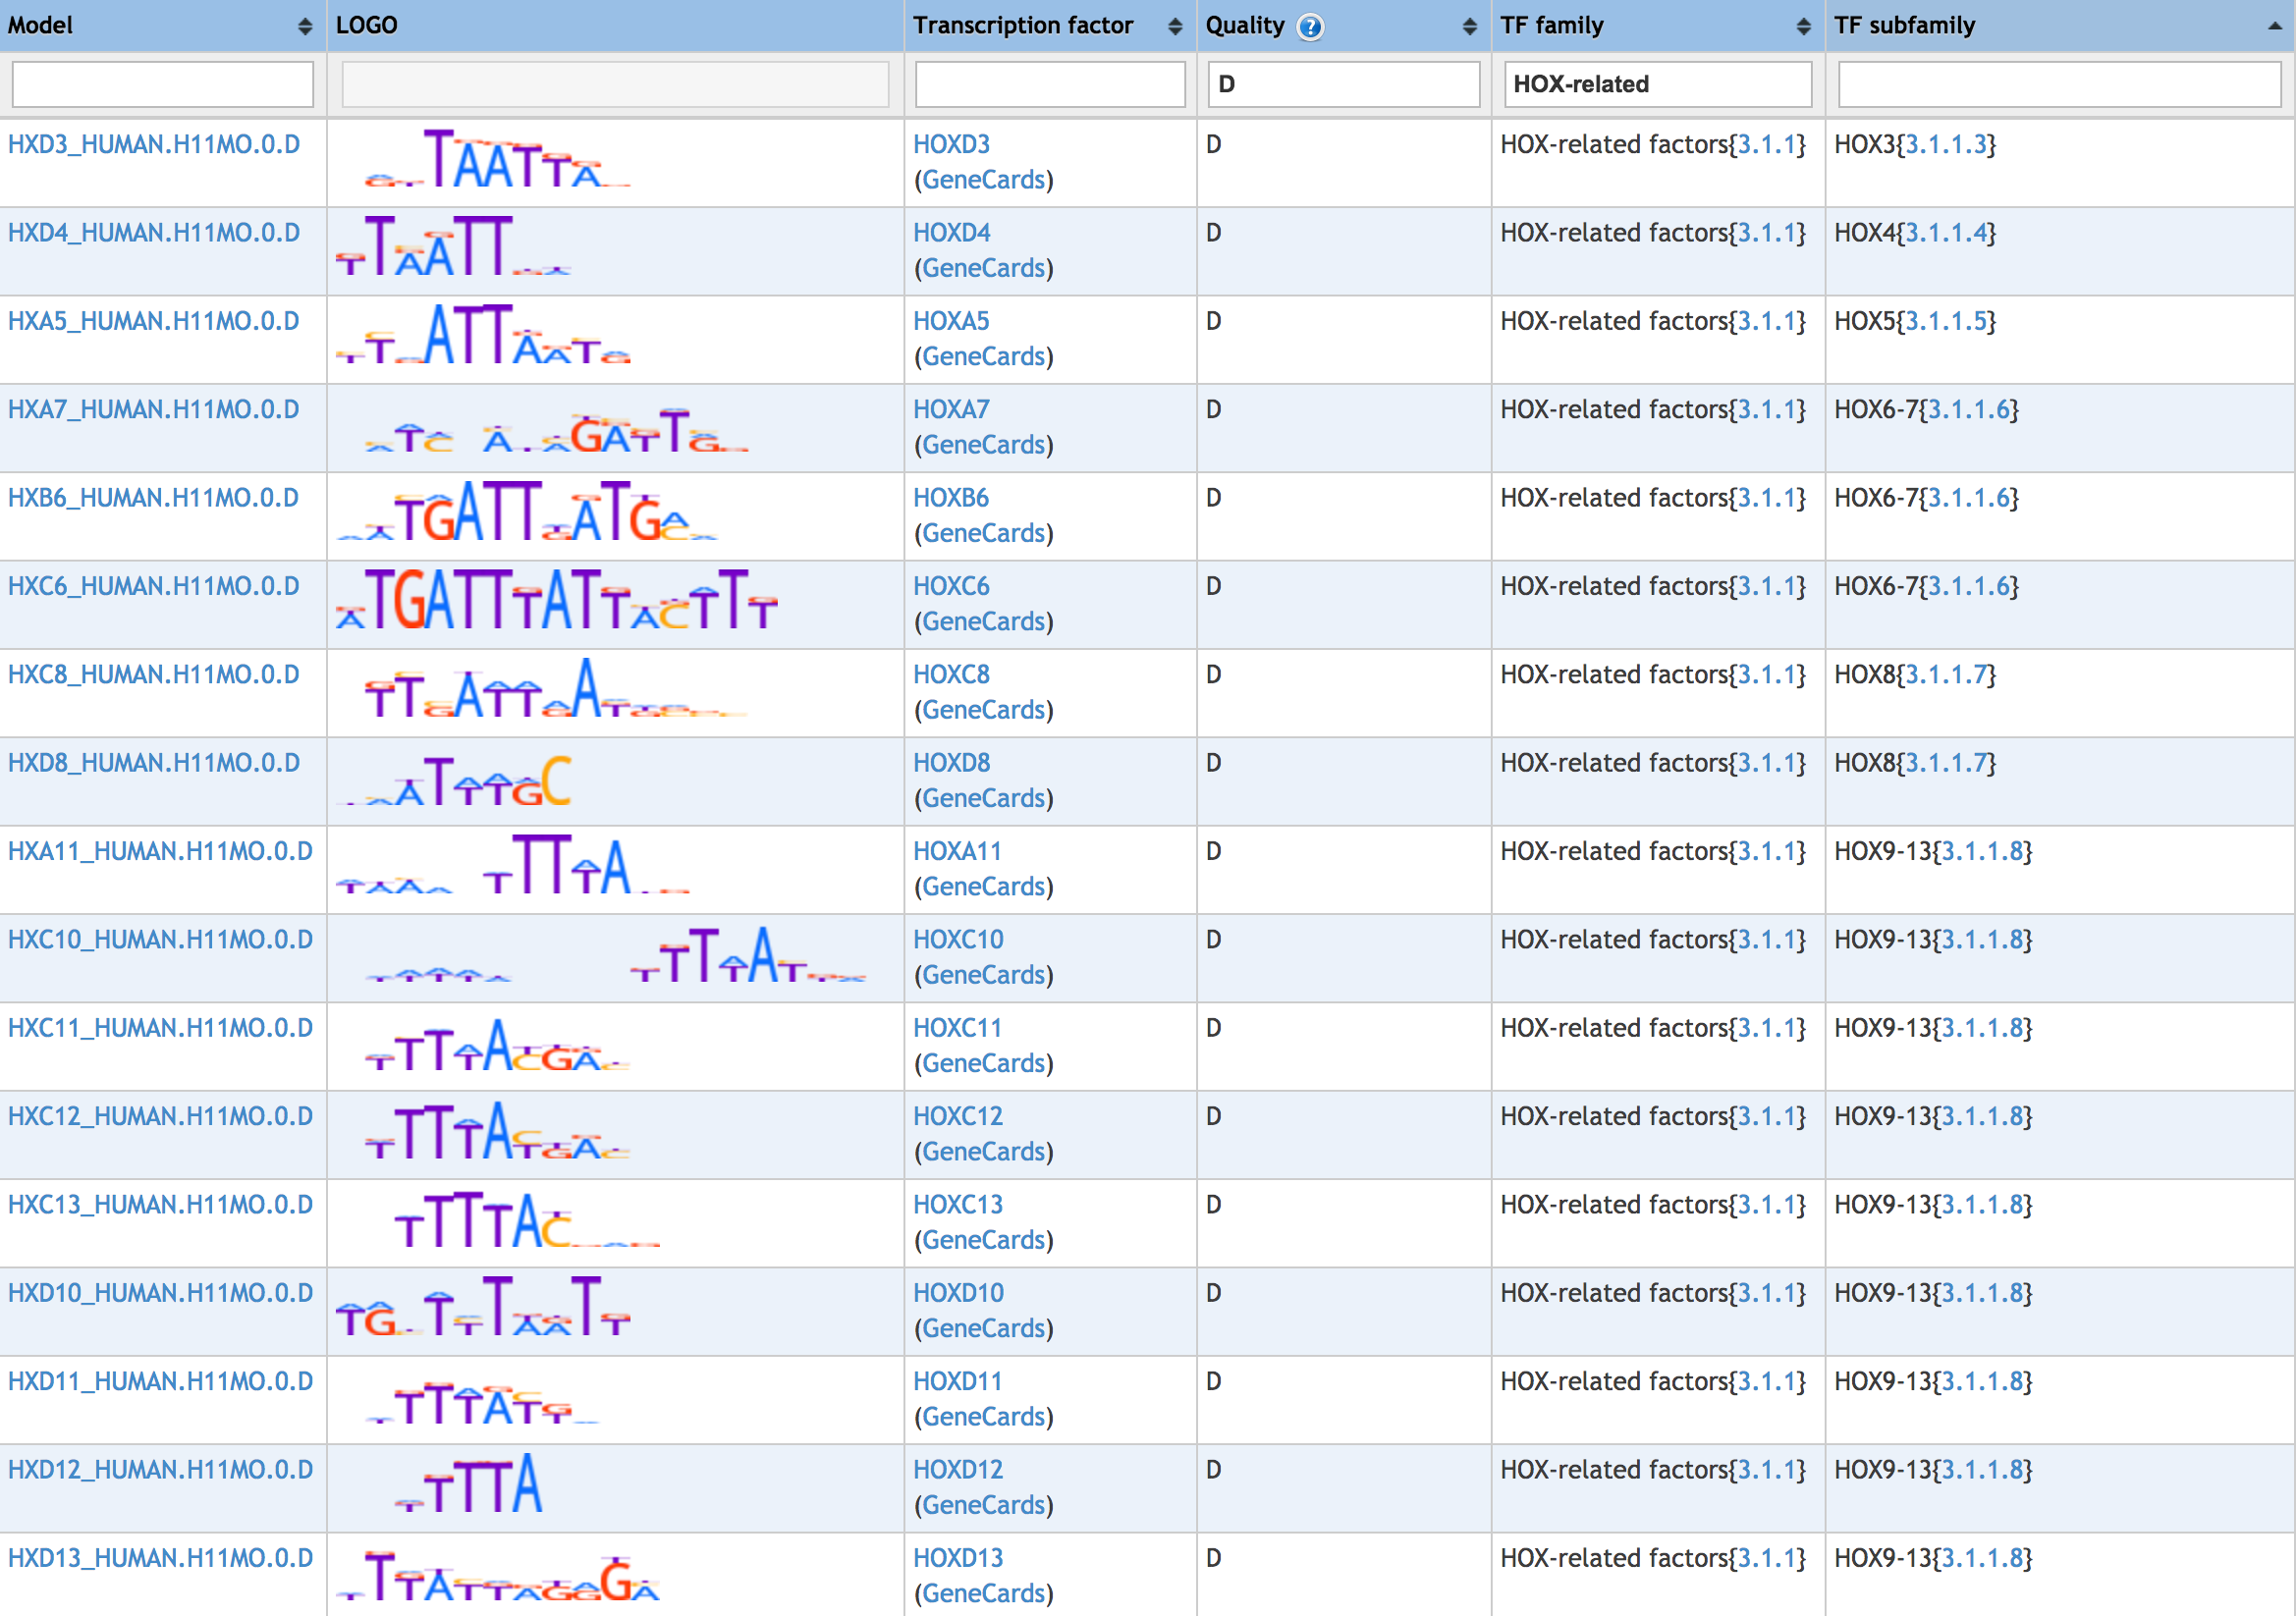
\includegraphics[width=16cm]{images/HOCOMOCO.png}
\caption[HOCOMOCO: HOX-related factors family]{\label{tab:hocomoco}HOCOMOCO V11: HOX-related factors family. Transcription factors HOXD13 and HOXD3 are in the same family (HOX-related factors) but in different subfamilies.}
\end{figure}

\end{center}

Overall, the results suggests that those regions that lost DNA methylation are bound by the regulatory TF Hmx3,
which  has been related to activation and maintenance of Gsh1 expression and subsequent downstream generation of \sigla{GHRH}{growth hormone-releasing hormone} expressing neurons \cite{morales2014regionalized} and \citeonline{pozsgai2010effect} conducted test with GHRH antagonists in glioblastoma cells showing efficacy of those drugs for experimental treatment of glioblastoma, HOXD13, which have been reported to be substantially up regulated in GBMs and may contribute to malignancy \cite{lee2015identification}, PAX3, which is essential for gliomagenesis \cite{xia2013pax3} also FOXM1  was shown by \citeonline{wang2015glioblastoma} to  promote the development and progression of GBM  and to be a novel therapeutic target against GBM.
To validate these findings, biological experiments are needed which by either knocking down these TFs or by regulating the DNA methylation levels of those binding regions will be able to verify if the downstream genes are being regulated.
